\documentclass[9pt]{beamer}
\mode<presentation>

% Theme choice:
\usetheme{Madrid}%Darmstadt 

\usecolortheme[RGB={0,100,50}]{structure}
 \usefonttheme{structurebold} 
\setbeamercovered{invisible}
%\setbeamertemplate{navigation symbols}{}
\usepackage{dynblocks}
\usepackage{textpos}
\usepackage{amsfonts}
\usepackage{amsmath}
\usepackage{amssymb}
\usepackage{amsthm}

\newtheorem{teorema}{Teorema}\usepackage{mathtools}
\renewcommand{\proofname}{Prova} 
\usepackage[portuguese]{babel}

\uselanguage{Portuguese}
\languagepath{Portuguese}

\deftranslation[to=Portuguese]{Theorem}{Teorema}
\deftranslation[to=Portuguese]{Lemma}{Lema}
\deftranslation[to=Portuguese]{Corollary}{Corolário}
\deftranslation[to=Portuguese]{Proof}{Prova}

\usepackage{dutchcal}
\usepackage{hyperref}
\usepackage[utf8]{inputenc}
\usepackage[T1]{fontenc}
\usepackage{amsthm}

\usepackage[affil-it]{authblk} 
\usepackage{etoolbox} 
\usepackage{lmodern}

% TikZ e CircuiTikZ
\usepackage{tikz}
\usepackage{circuitikz}
\usetikzlibrary{arrows.meta, positioning, circuits.logic.US, calc}
\makeatletter
\patchcmd{\@maketitle}{\LARGE \@title}{\fontsize{18}{19.2}\selectfont\@title}{}{}
\makeatother

\renewcommand\Authfont{\fontsize{12}{14.4}\selectfont}
\renewcommand\Affilfont{\fontsize{9}{10.8}\itshape}

% Title page details: 
\title[Presentation]{Lógica para Engenharia de Software} %add title


\institute[UniRV]{\textbf{\large  \textcolor{structure}{\textbf{\large
Álgebra Booleana
}}} %add name 
% \hspace{0.5pt}
\\ \qquad
\\Professor: Me. Sergio Souza Novak 
\\Faculdade de Engenharia de Software}

% \titlegraphic{\includegraphics[width=5cm]{msu.eps}}
\titlegraphic{
\includegraphics[width=5cm]{Universidade_de_Rio_Verde.jpg}}
\date{}

% Logo only on title page
%\logo{\includegraphics[width=1cm,keepaspectratio]{Logo.png}}
\usepackage[pscoord]{eso-pic}


\begin{document}

% Title page frame
\frame[plain]{\titlepage}
%logo
\AddToShipoutPictureFG{
    \put(\LenToUnit{.92\paperwidth},
    \LenToUnit{.185\paperheight})
    {\vtop{{\null}
    \makebox{
\includegraphics[width=.8cm,keepaspectratio]{Universidade_de_Rio_Verde.jpg}}}}}


\begin{frame}{Sumário}
  \tableofcontents
\end{frame}


% ============================================================
\section{1. Introdução e Conceitos Fundamentais}
% ============================================================

% -------------------------------------------------------
% SLIDE 1 — Motivação e Contexto Histórico
% -------------------------------------------------------
\begin{frame}{O que é a Álgebra Booleana?}

\begin{columns}

\column{0.55\textwidth}

\begin{block}{Definição}
A \textbf{Álgebra Booleana} é um sistema algébrico que opera sobre apenas \alert{dois valores}: \textbf{0} (falso) e \textbf{1} (verdadeiro).
\end{block}

\vspace{0.3cm}

\begin{block}{Contexto Histórico}
\begin{itemize}
    \item Criada por \textbf{George Boole} em 1854, na obra \textit{An Investigation of the Laws of Thought}.
    \item Em 1937, \textbf{Claude Shannon} aplicou-a ao projeto de circuitos digitais.
    \item Base matemática de todo hardware digital moderno.
\end{itemize}
\end{block}

\column{0.4\textwidth}

\begin{center}
\begin{tikzpicture}[scale=0.85]
  % Representação visual 0/1
  \draw[fill=green!20, draw=structure, thick, rounded corners=5pt]
    (0,0) rectangle (2.8,1.2);
  \node[font=\bfseries\Large, text=structure] at (1.4, 0.6) {0 \quad | \quad 1};
  \node[font=\tiny, text=gray] at (1.4, -0.3) {Falso \qquad Verdadeiro};

  \draw[fill=green!10, draw=structure, thick, rounded corners=5pt]
    (0, 1.9) rectangle (4.8, 4.2);
  \node[font=\small\bfseries, text=structure] at (1.4, 2.8) {Operações};
  \node[font=\small] at (2.8, 2.3) {AND $\cdot$ \quad OR $+$ \quad NOT $\overline{\phantom{x}}$};
\end{tikzpicture}
\end{center}

\end{columns}

\vspace{0.2cm}

\begin{alertblock}{Por que estudar?}
É a fundação da lógica digital, dos processadores e da simplificação de código.
\end{alertblock}

\end{frame}

% -------------------------------------------------------
% SLIDE 2 — Operações Fundamentais
% -------------------------------------------------------
\begin{frame}{Operações Fundamentais}

\begin{columns}

\column{0.48\textwidth}

\begin{block}{AND (Conjunção) — $A \cdot B$}
Resultado \textbf{1} somente se \textbf{ambas} as entradas forem 1.
\end{block}

\vspace{0.2cm}

\begin{block}{OR (Disjunção) — $A + B$}
Resultado \textbf{1} se \textbf{ao menos uma} entrada for 1.
\end{block}

\vspace{0.2cm}

\begin{block}{NOT (Negação) — $\overline{A}$}
\textbf{Inverte} o valor: 0 vira 1 e 1 vira 0.
\end{block}

\column{0.48\textwidth}

\begin{center}
\renewcommand{\arraystretch}{1.2}
\begin{tabular}{|c|c|c|c|c|}
\hline
$A$ & $B$ & $A \cdot B$ & $A + B$ & $\overline{A}$ \\
\hline
0 & 0 & \alert{0} & \alert{0} & 1 \\
0 & 1 & \alert{0} & \alert{1} & 1 \\
1 & 0 & \alert{0} & \alert{1} & 0 \\
1 & 1 & \alert{1} & \alert{1} & 0 \\
\hline
\end{tabular}

\vspace{0.4cm}

\begin{tikzpicture}[scale=0.9, font=\small]

  % ---------------- AND ----------------
  \node[and gate US, draw, thick, fill=green!10,
        logic gate inputs=nn, scale=1.1] (and1) at (0,0) {};

  % Entradas AND
  \draw (-1,0.3) -- (and1.input 1);
  \draw (-1,-0.3) -- (and1.input 2);

  \node[left] at (-1,0.3) {$A$};
  \node[left] at (-1,-0.3) {$B$};

  \node[right] at (and1.output) {\small AND};

  % ---------------- OR ----------------
  \node[or gate US, draw, thick, fill=blue!10,
        logic gate inputs=nn, scale=1.1] (or1) at (0,-1.8) {};

  % Entradas OR
  \draw (-1,-1.5) -- (or1.input 1);
  \draw (-1,-2.1) -- (or1.input 2);

  \node[left] at (-1,-1.5) {$A$};
  \node[left] at (-1,-2.1) {$B$};

  \node[right] at (or1.output) {\small OR};

  % ---------------- NOT ----------------
  \node[not gate US, draw, thick, fill=red!10,
        scale=1.1] (not1) at (0,-3.6) {};

  % Entrada NOT
  \draw (-1,-3.6) -- (not1.input);

  \node[left] at (-1,-3.6) {$A$};

  \node[right] at (not1.output) {\small NOT};

\end{tikzpicture}
\end{center}

\end{columns}

\end{frame}


% ============================================================
\section{4. Aplicações Práticas (Hardware e Software)}
\subsection{4.1. Hardware e Circuitos Digitais}

% -------------------------------------------------------
% SLIDE 4 — Portas Lógicas e Circuitos
% -------------------------------------------------------
\begin{frame}{Portas Lógicas em Circuitos Digitais}

\begin{block}{Portas Lógicas}
Cada operação booleana corresponde a um componente eletrônico chamado \textbf{porta lógica}, implementado com transistores.
\end{block}

\vspace{0.3cm}

\begin{center}
\begin{circuitikz}[scale=0.85, font=\small]

  % --- AND gate ---
  \node[and gate US, draw, thick, fill=green!10,
        logic gate inputs=nn, scale=1.2] (and1) at (0, 2) {};
  \draw (and1.input 1) -- ++(-0.8,0) node[left] {$A$};
  \draw (and1.input 2) -- ++(-0.8,0) node[left] {$B$};
  \draw (and1.output) -- ++(0.6,0) node[right] {$S = A{\cdot}B$};
  \node[below=0.05cm of and1, font=\footnotesize, text=gray] {AND};

  % --- OR gate ---
  \node[or gate US, draw, thick, fill=blue!10,
        logic gate inputs=nn, scale=1.2] (or1) at (4.5, 2) {};
  \draw (or1.input 1) -- ++(-0.8,0) node[left] {$A$};
  \draw (or1.input 2) -- ++(-0.8,0) node[left] {$B$};
  \draw (or1.output) -- ++(0.6,0) node[right] {$S = A{+}B$};
  \node[below=0.05cm of or1, font=\footnotesize, text=gray] {OR};

  % --- NOT gate ---
  \node[not gate US, draw, thick, fill=orange!10,
        scale=1.2] (not1) at (2.2, 0.2) {};
  \draw (not1.input) -- ++(-0.8,0) node[left] {$A$};
  \draw (not1.output) -- ++(0.6,0) node[right] {$S = \overline{A}$};
  \node[below=0.05cm of not1, font=\footnotesize, text=gray] {NOT};

  % --- NAND gate ---
  \node[nand gate US, draw, thick, fill=red!10,
        logic gate inputs=nn, scale=1.2] (nand1) at (4.5, 0.2) {};
  \draw (nand1.input 1) -- ++(-0.8,0) node[left] {$A$};
  \draw (nand1.input 2) -- ++(-0.8,0) node[left] {$B$};
  \draw (nand1.output) -- ++(0.6,0) node[right] {$S = \overline{A{\cdot}B}$};
  \node[below=0.05cm of nand1, font=\footnotesize, text=gray] {NAND};

\end{circuitikz}
\end{center}

\vspace{0.1cm}
\textcolor{gray}{\footnotesize Transistores BJT e CMOS implementam essas portas em silício.}

\end{frame}

% -------------------------------------------------------
% SLIDE 5 — Componentes Físicos e Implementação Real
% -------------------------------------------------------
\begin{frame}{Componentes Físicos e Implementação Real}

\begin{columns}

\column{0.3\textwidth}
\begin{block}{Hardware no "Mundo Real"}
Na prática, as portas lógicas são encontradas em \textbf{Circuitos Integrados (CIs)}, como a famosa série 7400.
\begin{itemize}
    \item \textbf{Encapsulamento:} Proteção física e pinagem padrão.
    \item \textbf{Miniaturização:} Bilhões de portas em um chip.
    \item \textbf{Sinais Elétricos:} 0 (GND) e 1 ($V_{CC}$).
\end{itemize}
\end{block}

\column{0.68\textwidth}
\begin{center}
    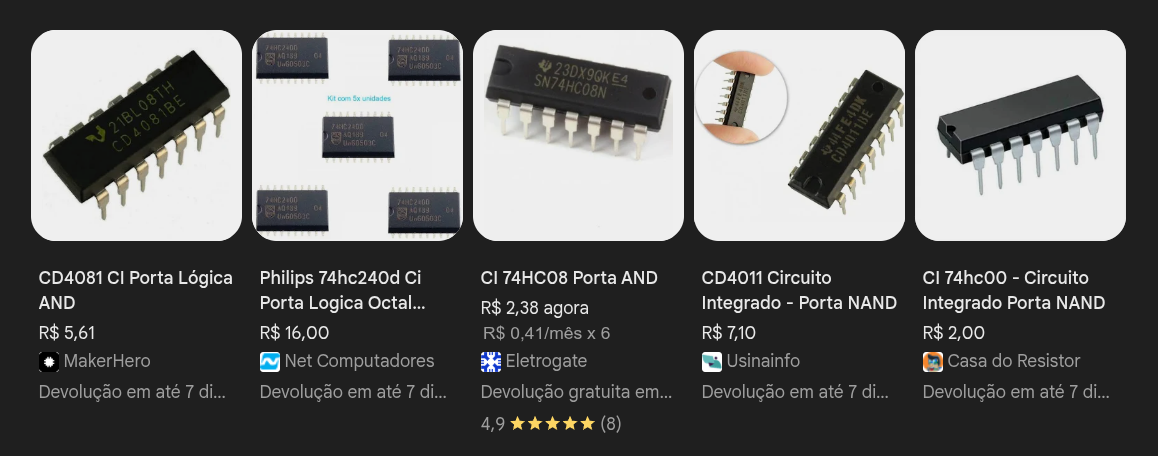
\includegraphics[width=\textwidth]{portasfisicas.png}
    \vspace{0.1cm}
    \textcolor{gray}{\footnotesize Exemplo de CIs com portas lógicas discretas.}
\end{center}

\end{columns}

\begin{alertblock}{Aplicações Móveis e Industriais}
Desde o controle de um semáforo até a lógica de execução de um smartphone, tudo depende da orquestração física desses componentes.
\end{alertblock}

\end{frame}

% -------------------------------------------------------
% SLIDE 6 — Aplicação Prática: Display de 7 Segmentos
% -------------------------------------------------------
\begin{frame}{Aplicação Prática: Display de 7 Segmentos}

\begin{columns}

\column{0.4\textwidth}
\begin{block}{O que é?}
Um componente eletrônico comum usado para exibir numerais decimais.
\end{block}

\begin{itemize}
    \item Composto por 7 LEDs (segmentos de \textbf{a} até \textbf{g}).
    \item Cada segmento é controlado de forma independente.
    \item Um dos maiores exemplos de uso de \textbf{Lógica Combinacional}.
\end{itemize}

\column{0.58\textwidth}
\begin{center}
    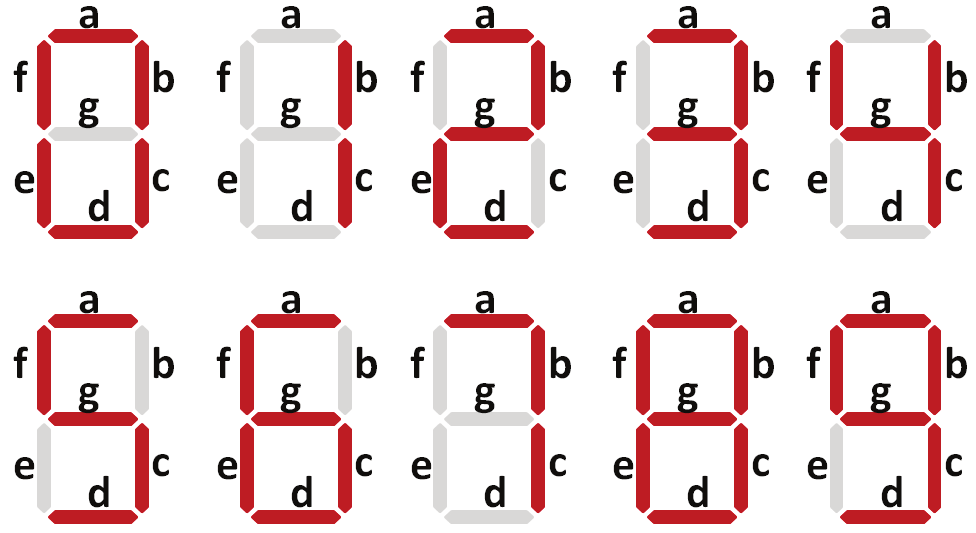
\includegraphics[width=0.7\textwidth]{display7.png}
    \vspace{0.2cm}
    \textcolor{gray}{\footnotesize Estrutura de segmentos (a-g).}
\end{center}

\end{columns}

\end{frame}

% -------------------------------------------------------
% SLIDE 7 — Como funciona a decodificação?
% -------------------------------------------------------
\begin{frame}{Como funciona a decodificação?}

\begin{block}{A Lógica por trás dos Números}
Para cada número que queremos exibir, precisamos de uma \textbf{expressão booleana} específica para cada segmento.
\end{block}

\begin{center}
    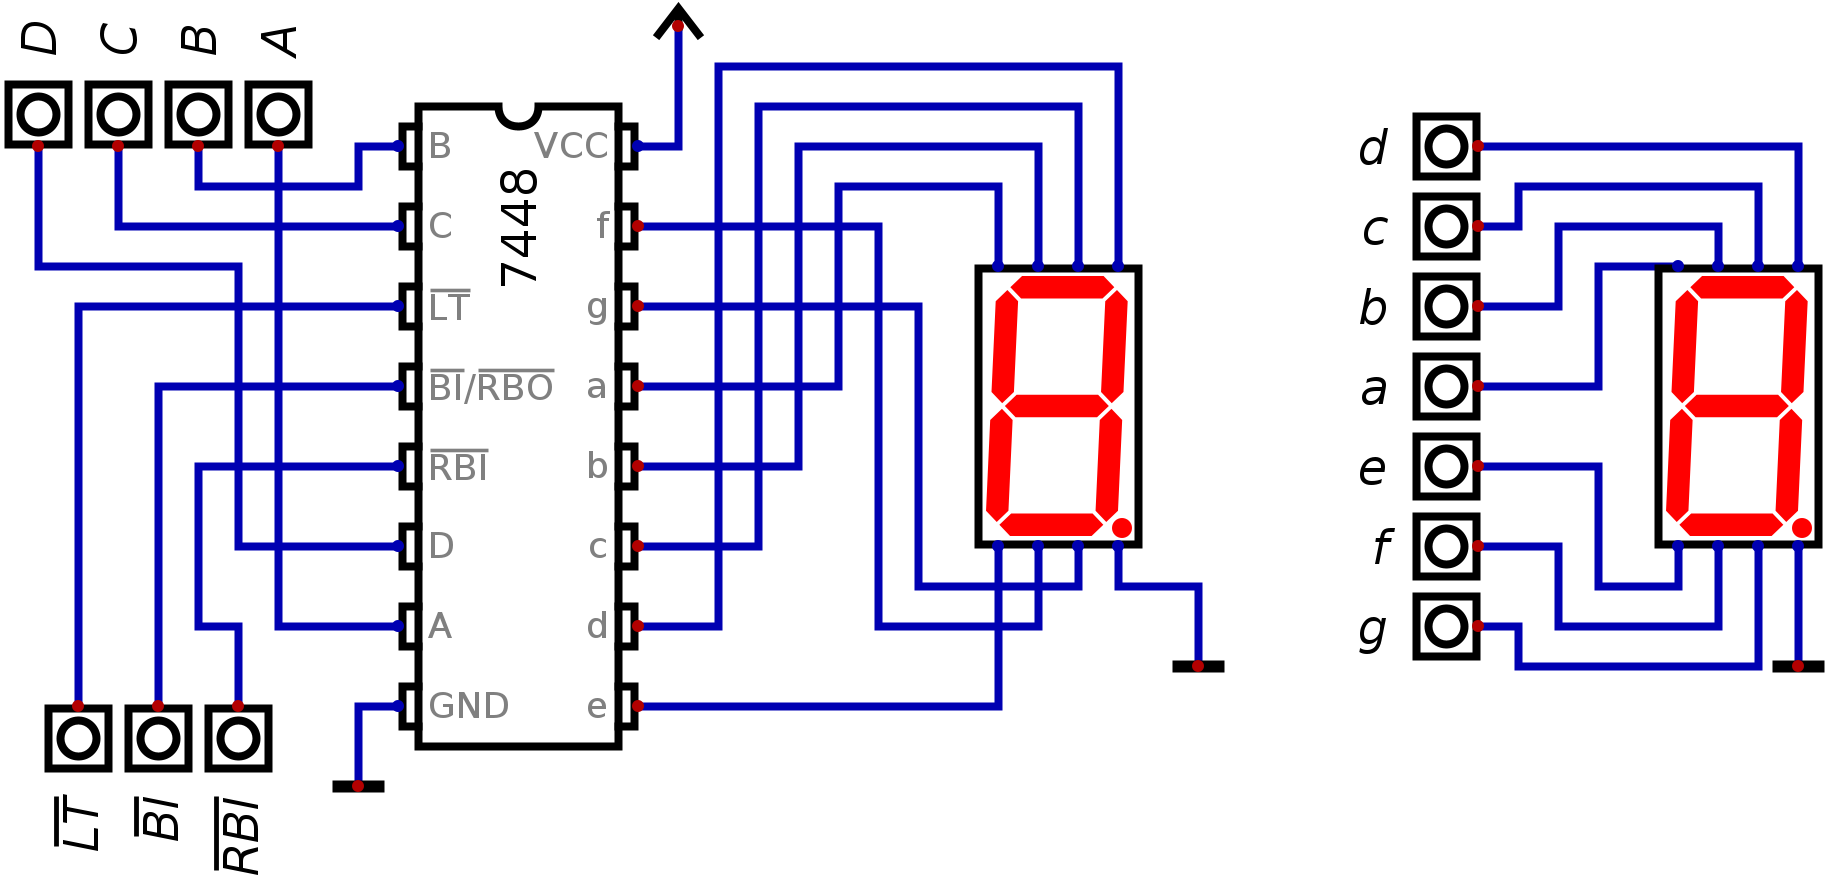
\includegraphics[width=0.7\textwidth]{display7_usage.png}
\end{center}

\begin{exampleblock}{Exemplo: O número "1"}
Para formar o número "1", os segmentos \textbf{b} e \textbf{c} devem ser 1 (LIGADOS), enquanto \textbf{a, d, e, f, g} devem ser 0 (DESLIGADOS).
\end{exampleblock}

\end{frame}

% -------------------------------------------------------
% SLIDE 8 — Implementação com Portas Lógicas
% -------------------------------------------------------
\begin{frame}{Implementação com Portas Lógicas}

\begin{block}{O Decodificador de 7 Segmentos}
Um circuito digital recebe um número em binário (ex: 4 bits) e ativa os segmentos correspondentes através de uma rede de portas lógicas.
\end{block}

\begin{center}
    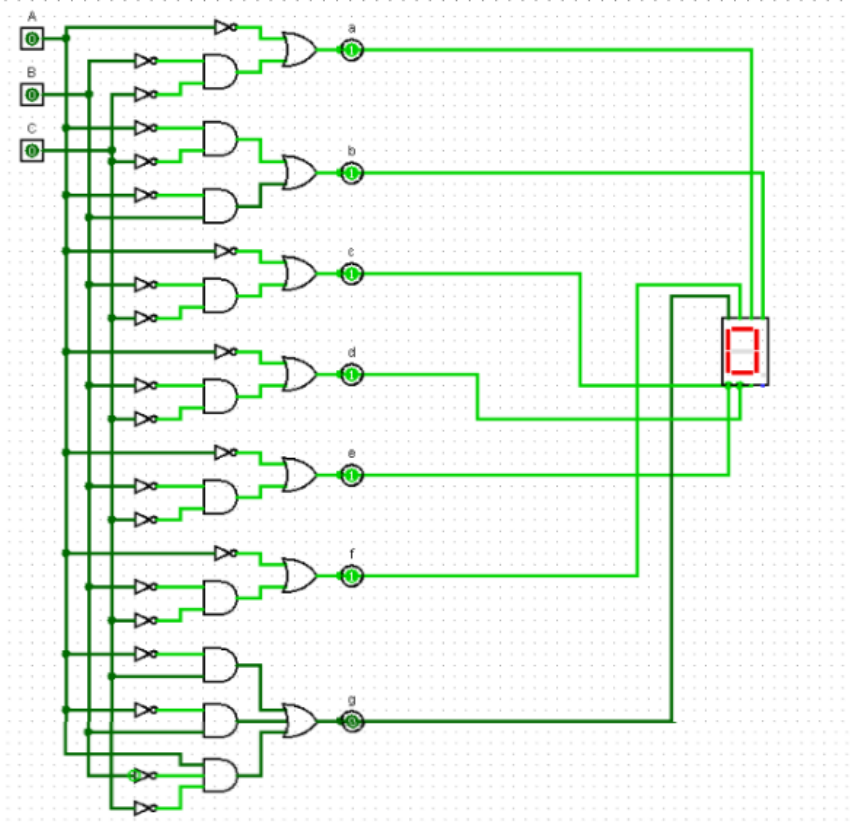
\includegraphics[width=0.45\textwidth]{display_7_portas_logicas.png}
\end{center}

\textcolor{structure}{\footnotesize \textbf{Nota:} A simplificação booleana aqui é CRUCIAL para reduzir o número de transistores no chip.}

\end{frame}
% -------------------------------------------------------
% SLIDE 6 — Simplificação Algébrica (com circuitos)
% -------------------------------------------------------
\begin{frame}[fragile]{Simplificação Algébrica}

\begin{block}{Exemplo}
Simplificar $F = A\overline{B} + AB$
\end{block}

\vspace{0.2cm}

\begin{columns}

% ================= COLUNA 1 =================
\column{0.48\textwidth}

\begin{block}{Circuito original}
\begin{center}
\begin{tikzpicture}[circuit logic US, scale=0.9, font=\scriptsize]

  % Entradas
  \node at (-2,1) {$A$};
  \node at (-2,-1) {$B$};

  % Linhas de entrada
  \draw (-1.8,1) -- (-1,1);
  \draw (-1.8,-1) -- (-1,-1);

  % NOT em B
  \node[not gate, draw] (notB) at (-0.5,-1.4) {};
  \draw (-1,-1) -- (notB.input);

  % AND superior (A AND NOT B)
  \node[and gate, draw] (and1) at (1,0.7) {};
  \draw (-1,1) |- (and1.input 1);
  \draw (notB.output) |- (and1.input 2);

  % AND inferior (A AND B)
  \node[and gate, draw] (and2) at (1,-0.7) {};
  \draw (-1,1) |- (and2.input 1);
  \draw (-1,-1) |- (and2.input 2);

  % OR final
  \node[or gate, draw] (or1) at (3,0) {};
  \draw (and1.output) -- (or1.input 1);
  \draw (and2.output) -- (or1.input 2);

  % Saída
  \draw (or1.output) -- (4,0);
  \node at (4.3,0) {$F$};

\end{tikzpicture}

\vspace{0.2cm}
\textcolor{red}{\tiny 4 portas: 2 AND + 1 OR + 1 NOT}
\end{center}
\end{block}

% ================= COLUNA 2 =================
\column{0.48\textwidth}

\begin{block}{Circuito simplificado}
\begin{center}
\begin{tikzpicture}[scale=0.9, font=\scriptsize]

  % Entrada A
  \node at (-2,0) {$A$};

  % Fio direto
  \draw (-1.8,0) -- (2,0);

  % Saída
  \node at (2.3,0) {$F$};

\end{tikzpicture}

\vspace{0.2cm}
\textcolor{green!60!black}{\tiny Sem portas — conexão direta}
\end{center}
\end{block}

\end{columns}

\vspace{0.3cm}

\begin{alertblock}{Resultado}
\[
F = A
\]
\end{alertblock}

\end{frame}

% ============================================================
\section{3. Técnicas de Simplificação Booleana}
% ============================================================

% -------------------------------------------------------
% SLIDE 6 — Simplificação Algébrica
% -------------------------------------------------------
\begin{frame}{Simplificação Algébrica}

\begin{block}{Objetivo}
Reduzir uma expressão booleana ao menor número de operações, economizando \alert{portas lógicas} no hardware ou \alert{condicionais} no código.
\end{block}

\vspace{0.2cm}

\textbf{Exemplo: Simplificar $F = A\overline{B} + AB$}

\vspace{0.1cm}

\begin{columns}

\column{\textwidth}

\begin{block}{Circuito original vs. simplificado}
\begin{center}
\begin{tikzpicture}[font=\footnotesize, scale=0.85]
  % Original
  \node[fill=red!15, rounded corners, draw=red, thick,
        minimum width=2.4cm, minimum height=0.7cm]
    at (1.2, 1.2) {$A\overline{B} + AB$};
  \node[text=red, font=\tiny] at (1.2, 0.75) {3 portas lógicas};

  % Seta
  \draw[->, thick, draw=structure] (1.2, 0.55) -- (1.2, -0.05);

  % Simplificado
  \node[fill=green!15, rounded corners, draw=structure, thick,
        minimum width=2.4cm, minimum height=0.7cm]
    at (1.2, -0.3) {$A$};
  \node[text=structure, font=\tiny] at (1.2, -0.75) {0 portas — apenas fio!};
\end{tikzpicture}
\end{center}
\end{block}

\end{columns}

\end{frame}

% -------------------------------------------------------
% SLIDE 6b — Simplificação de Circuito com 3 Variáveis
% -------------------------------------------------------
\begin{frame}[fragile]{Simplificação de Circuito com 3 Variáveis}

\begin{block}{Problema}
Simplificar a expressão: $F = AB + A\overline{C} + B\overline{C}$
\end{block}

\vspace{0.15cm}

\begin{columns}
\column{\textwidth}

\begin{block}{Circuito original — 5 portas}
\begin{center}
\begin{circuitikz}[scale=0.62, font=\scriptsize, transform shape]

  % Entradas
  \node (A)  at (-3.5, 3.8) {$A$};
  \node (B)  at (-3.5, 2.3) {$B$};
  \node (nC) at (-3.5, 0.8) {$\overline{C}$};

  % AND1: A AND B
  \node[and gate US, draw, thick, fill=green!10,
        logic gate inputs=nn, scale=1.0] (and1) at (0, 3.2) {};
  \draw (A.east)  -- ++(0.4,0) |- (and1.input 1);
  \draw (B.east)  -- ++(0.2,0) |- (and1.input 2);
  \draw (and1.output) -- ++(0.3,0) node[right, xshift=1pt] {\tiny $AB$};

  % AND2: A AND NOT(C)
  \node[and gate US, draw, thick, fill=green!10,
        logic gate inputs=nn, scale=1.0] (and2) at (0, 2.0) {};
  \draw (A.east)  -- ++(0.4,0) |- (and2.input 1);
  \draw (nC.east) -- ++(0.2,0) |- (and2.input 2);
  \draw (and2.output) -- ++(0.3,0) node[right, xshift=1pt] {\tiny $A\overline{C}$};

  % AND3: B AND NOT(C)
  \node[and gate US, draw, thick, fill=red!10,
        logic gate inputs=nn, scale=1.0] (and3) at (0, 0.8) {};
  \draw (B.east)  -- ++(0.2,0) |- (and3.input 1);
  \draw (nC.east) -- ++(0.2,0) |- (and3.input 2);
  \draw (and3.output) -- ++(0.3,0) node[right, xshift=1pt] {\tiny $B\overline{C}$};

  % OR de 3 entradas via OR aninhado
  \node[or gate US, draw, thick, fill=blue!10,
        logic gate inputs=nn, scale=1.0] (or1) at (3.2, 2.5) {};
  \draw (and1.output) ++(0.3,0) -- ++(0.2,0) |- (or1.input 1);
  \draw (and2.output) ++(0.3,0) -- ++(0.2,0) |- (or1.input 2);

  \node[or gate US, draw, thick, fill=blue!10,
        logic gate inputs=nn, scale=1.0] (or2) at (4.8, 1.8) {};
  \draw (or1.output) |- (or2.input 1);
  \draw (and3.output) ++(0.3,0) -- ++(0.8,0) |- (or2.input 2);
  \draw (or2.output) -- ++(0.4,0) node[right] {$F$};

\end{circuitikz}
\end{center}
\end{block}

\vspace{0.1cm}

\begin{block}{Circuito simplificado — 3 portas}
\begin{center}
\begin{circuitikz}[scale=0.65, font=\scriptsize, transform shape]

  \node (A)  at (-2.5, 2.2) {$A$};
  \node (B)  at (-2.5, 1.2) {$B$};
  \node (nC) at (-2.5, 0.2) {$\overline{C}$};

  \node[and gate US, draw, thick, fill=green!10,
        logic gate inputs=nn, scale=1.0] (and1) at (0.2, 1.9) {};
  \draw (A.east) -- ++(0.3,0) |- (and1.input 1);
  \draw (B.east) -- ++(0.2,0) |- (and1.input 2);

  \node[and gate US, draw, thick, fill=green!10,
        logic gate inputs=nn, scale=1.0] (and2) at (0.2, 0.6) {};
  \draw (A.east)  -- ++(0.3,0) |- (and2.input 1);
  \draw (nC.east) -- ++(0.2,0) |- (and2.input 2);

  \node[or gate US, draw, thick, fill=blue!10,
        logic gate inputs=nn, scale=1.0] (or1) at (2.6, 1.2) {};
  \draw (and1.output) |- (or1.input 1);
  \draw (and2.output) |- (or1.input 2);
  \draw (or1.output) -- ++(0.4,0) node[right] {$F$};

\end{circuitikz}
\end{center}
\textcolor{structure}{\footnotesize \textbf{Redução:} 5 portas $\rightarrow$ 3 portas (40\%)}
\end{block}

\end{columns}

\end{frame}

% ============================================================
\subsection{4.2. Lógica de Programação e Software}
% ============================================================

% -------------------------------------------------------
% SLIDE 7 — Simplificação de Condicionais em Código
% -------------------------------------------------------
\begin{frame}[fragile]{Simplificação de Condicionais em Código}

\begin{block}{Conexão direta}
Toda condição lógica em código (\texttt{if}, \texttt{while}, \texttt{assert}) é uma \textbf{expressão booleana}. Simplificá-la reduz complexidade e elimina bugs.
\end{block}

\vspace{0.2cm}

\begin{columns}

\column{0.48\textwidth}

\begin{alertblock}{Código redundante}
\begin{verbatim}
if (autenticado == true
    && autenticado == true) {
    acessar();
}
\end{verbatim}
Expressão: $A \cdot A = A$

\vspace{0.1cm}
\textcolor{red}{Idempotência violada!}
\end{alertblock}

\column{0.48\textwidth}

\begin{block}{Código simplificado}
\begin{verbatim}
if (autenticado) {
    acessar();
}
\end{verbatim}
Expressão: $A$

\vspace{0.1cm}
\textcolor{structure}{Limpo e correto.}
\end{block}

\end{columns}

\vspace{0.3cm}

\begin{block}{Outro exemplo — De Morgan}
\begin{center}
\texttt{!(A \&\& B)} $\equiv$ \texttt{!A || !B}
\qquad {\footnotesize (Teorema de De Morgan)}
\end{center}
Muito usado para inverter guardas em loops e simplificar condições de saída.
\end{block}

\end{frame}

% -------------------------------------------------------
% SLIDE 7b — Refatoração de Lógica Complexa
% -------------------------------------------------------
\begin{frame}[fragile]{Refatoração de Lógica Complexa}

\begin{block}{Exemplo: Regra de Negócio para Desconto}
Imagine um sistema onde um desconto é aplicado se o usuário é Administrador E Dono da conta E tem um Cupom, OU se ele é Administrador E NÃO é Dono E tem um Cupom.
\end{block}

\begin{columns}

\column{0.55\textwidth}

\begin{alertblock}{Código sem simplificação}
\begin{verbatim}
if ((isAdmin && isOwner && hasVoucher) 
 || (isAdmin && !isOwner && hasVoucher)) {
    aplicarDesconto();
}
\end{verbatim}
\end{alertblock}

\column{0.41\textwidth}

\begin{block}{Aplicação da Álgebra}
$A = \texttt{isAdmin}$

$B = \texttt{isOwner}$

$C = \texttt{hasVoucher}$

\vspace{0.2cm}
$A \cdot B \cdot C + A \cdot \overline{B} \cdot C$
$= A \cdot C \cdot (B + \overline{B})$
$= A \cdot C \cdot 1$
$= \boxed{A \cdot C}$
\end{block}

\end{columns}

\vspace{0.2cm}

\begin{block}{Código Refatorado (Equivalente)}
\begin{verbatim}
if (isAdmin && hasVoucher) {
    aplicarDesconto();
}
\end{verbatim}
\textcolor{structure}{\footnotesize \textbf{Resultado:} A variável \texttt{isOwner} é \alert{irrelevante} para o resultado final desta condição.}
\end{block}

\end{frame}

% ============================================================
\section{2. Propriedades e Teoremas Fundamentais}
% ============================================================

% -------------------------------------------------------
% LEIS DE IDENTIDADE
% -------------------------------------------------------
\begin{frame}[fragile]{1. Leis de Identidade}

\begin{block}{Propriedade: Elemento Neutro}
\[ A + 0 = A \qquad \text{e} \qquad A \cdot 1 = A \]
\end{block}

\begin{columns}

\column{0.48\textwidth}
\begin{block}{Visão de Circuito (OR)}
\begin{center}
\begin{circuitikz}[scale=0.7, transform shape]
  \node[or gate US, draw, thick] (or1) at (0,0) {};
  \draw (or1.input 1) -- ++(-0.5,0) node[left] {$A$};
  \draw (or1.input 2) -- ++(-0.5,0) node[left] {$0$ (GND)};
  \draw (or1.output) -- ++(0.5,0) node[right] {$F = A$};
\end{circuitikz}
\end{center}
\textcolor{structure}{\footnotesize \textbf{Simplificação:} A porta OR é desnecessária; basta o fio de $A$.}
\end{block}

\column{0.48\textwidth}
\begin{block}{Visão de Código (if)}
\begin{verbatim}
// Inicial
if (A || false) { ... }

// Simplificado
if (A) { ... }
\end{verbatim}
\textcolor{structure}{\footnotesize O valor constante não altera o resultado de $A$.}
\end{block}

\end{columns}

\end{frame}

% -------------------------------------------------------
% LEIS DE NULIDADE
% -------------------------------------------------------
\begin{frame}[fragile]{2. Leis de Nulidade}

\begin{block}{Propriedade: Elemento Dominante}
\[ A + 1 = 1 \qquad \text{e} \qquad A \cdot 0 = 0 \]
\end{block}

\begin{columns}

\column{0.48\textwidth}
\begin{block}{Visão de Circuito (AND)}
\begin{center}
\begin{circuitikz}[scale=0.7, transform shape]
  \node[and gate US, draw, thick] (and1) at (0,0) {};
  \draw (and1.input 1) -- ++(-0.5,0) node[left] {$A$};
  \draw (and1.input 2) -- ++(-0.5,0) node[left] {$0$ (GND)};
  \draw (and1.output) -- ++(0.5,0) node[right] {$F = 0$};
\end{circuitikz}
\end{center}
\textcolor{red}{\footnotesize \textbf{Simplificação:} A saída é sempre 0, independente de $A$.}
\end{block}

\column{0.48\textwidth}
\begin{block}{Visão de Código (if)}
\begin{verbatim}
// Inicial
if (A && false) { ... }

// Simplificado
// (Código inacessível)
\end{verbatim}
\textcolor{red}{\footnotesize O compilador pode remover este bloco (\textit{Dead Code}).}
\end{block}

\end{columns}

\end{frame}

% -------------------------------------------------------
% LEIS DE IDEMPOTÊNCIA
% -------------------------------------------------------
\begin{frame}[fragile]{3. Leis de Idempotência}

\begin{block}{Propriedade: Repetição}
\[ A + A = A \qquad \text{e} \qquad A \cdot A = A \]
\end{block}

\begin{columns}

\column{0.48\textwidth}
\begin{block}{Visão de Circuito}
\begin{center}
\begin{circuitikz}[scale=0.7, transform shape]
  \node[or gate US, draw, thick] (or1) at (0,0) {};
  \draw (or1.input 1) -- ++(-0.5,0) node (in1) {};
  \draw (or1.input 2) -- ++(-0.5,0) node (in2) {};
  \draw (in1.center) node[circle,fill,inner sep=1pt] {} |- (in2.center);
  \draw (in1.center) -- ++(-0.3,0) node[left] {$A$};
  \draw (or1.output) -- ++(0.5,0) node[right] {$F = A$};
\end{circuitikz}
\end{center}
\textcolor{structure}{\footnotesize Comparar o mesmo sinal consigo mesmo é redundante.}
\end{block}

\column{0.48\textwidth}
\begin{block}{Visão de Código (if)}
\begin{verbatim}
// Inicial
if (A || A) { ... }

// Simplificado
if (A) { ... }
\end{verbatim}
\textcolor{structure}{\footnotesize Ocorre frequentemente em lógicas de filtros complexos.}
\end{block}

\end{columns}

\end{frame}

% -------------------------------------------------------
% LEIS DO COMPLEMENTO
% -------------------------------------------------------
\begin{frame}[fragile]{4. Leis do Complemento}

\begin{block}{Propriedade: Inversa}
\[ A + \overline{A} = 1 \qquad \text{e} \qquad A \cdot \overline{A} = 0 \]
\end{block}

\begin{columns}

\column{0.48\textwidth}
\begin{block}{Visão de Circuito}
\begin{center}
\begin{circuitikz}[scale=0.7, transform shape]
  \node[and gate US, draw, thick] (and1) at (1.5,0) {};
  \node[not gate US, draw, thick] (not1) at (0,-0.28) {};
  \draw (and1.input 1) -- ++(-1.8,0) node[left] {$A$} node(pt){};
  \draw (and1.input 2) -- (not1.output);
  \draw (pt.center) node[circle,fill,inner sep=1pt] {} |- (not1.input);
  \draw (and1.output) -- ++(0.5,0) node[right] {$F = 0$};
\end{circuitikz}
\end{center}
\end{block}

\column{0.48\textwidth}
\begin{block}{Visão de Código (if)}
\begin{verbatim}
// Inicial
if (A && !A) { ... }

// Simplificado
// Nunca executa
\end{verbatim}
\textcolor{red}{\footnotesize Uma variável não pode ser verdadeira e falsa ao mesmo tempo.}
\end{block}

\end{columns}

\end{frame}

% -------------------------------------------------------
% LEI DA DUPLA NEGAÇÃO
% -------------------------------------------------------
\begin{frame}[fragile]{5. Lei da Dupla Negação}

\begin{block}{Propriedade: Involução}
\[ \overline{\overline{A}} = A \]
\end{block}

\begin{columns}

\column{0.48\textwidth}
\begin{block}{Visão de Circuito}
\begin{center}
\begin{circuitikz}[scale=0.8, transform shape]
  \node[not gate US, draw, thick] (not1) at (0,0) {};
  \node[not gate US, draw, thick] (not2) at (1.5,0) {};
  \draw (not1.input) -- ++(-0.5,0) node[left] {$A$};
  \draw (not1.output) -- (not2.input);
  \draw (not2.output) -- ++(0.5,0) node[right] {$F = A$};
\end{circuitikz}
\end{center}
\textcolor{structure}{\footnotesize Duas inversões seguidas retornam ao valor original.}
\end{block}

\column{0.48\textwidth}
\begin{block}{Visão de Código (if)}
\begin{verbatim}
// Inicial
if (!!A) { ... }

// Simplificado
if (A) { ... }
\end{verbatim}
\textcolor{structure}{\footnotesize Comum em JavaScript para converter valores para booleano, mas logicamente redundante.}
\end{block}

\end{columns}

\end{frame}

% -------------------------------------------------------
% LEIS COMUTATIVAS
% -------------------------------------------------------
\begin{frame}[fragile]{6. Leis Comutativas}

\begin{block}{Propriedade: Troca de Ordem}
\[ A + B = B + A \qquad \text{e} \qquad A \cdot B = B \cdot A \]
\end{block}

\begin{columns}

\column{0.48\textwidth}
\begin{block}{Visão de Circuito}
\begin{center}
\begin{circuitikz}[scale=0.7, transform shape]
  \node[and gate US, draw, thick] (and1) at (0,0) {};
  \draw (and1.input 1) -- ++(-0.5,0) node[left] {$A$};
  \draw (and1.input 2) -- ++(-0.5,0) node[left] {$B$};
  \draw (and1.output) -- ++(0.5,0) node[right] {$F = AB$};
\end{circuitikz}
\end{center}
\textcolor{structure}{\footnotesize A ordem das entradas não altera o resultado da porta lógica.}
\end{block}

\column{0.48\textwidth}
\begin{block}{Visão de Código (if)}
\begin{verbatim}
// Caso 1
if (A && B) { ... }

// Caso 2 (Equivalente)
if (B && A) { ... }
\end{verbatim}
\textcolor{structure}{\footnotesize \textbf{Nota:} Em linguagens com \textit{short-circuit}, a ordem pode afetar a performance.}
\end{block}

\end{columns}

\end{frame}

% -------------------------------------------------------
% LEIS ASSOCIATIVAS
% -------------------------------------------------------
\begin{frame}[fragile]{7. Leis Associativas}

\begin{block}{Propriedade: Agrupamento}
\[ (A + B) + C = A + (B + C) \]
\[ (A \cdot B) \cdot C = A \cdot (B \cdot C) \]
\end{block}

\begin{columns}

\column{0.48\textwidth}
\begin{block}{Visão de Circuito (AND)}
\begin{center}
\begin{circuitikz}[scale=0.6, transform shape]
  \node[and gate US, draw, thick] (and1) at (0,1) {};
  \node[and gate US, draw, thick] (and2) at (1.5,0.5) {};
  \draw (and1.input 1) -- ++(-0.5,0) node[left] {$A$};
  \draw (and1.input 2) -- ++(-0.5,0) node[left] {$B$};
  \draw (and1.output) |- (and2.input 1);
  \draw (and2.input 2) -- ++(-2,0) node[left] {$C$};
  \draw (and2.output) -- ++(0.5,0) node[right] {$F = (AB)C$};
\end{circuitikz}
\end{center}
\end{block}

\column{0.48\textwidth}
\begin{block}{Visão de Código (if)}
\begin{verbatim}
// Inicial
if ((A && B) && C) { ... }

// Simplificado
if (A && B && C) { ... }
\end{verbatim}
\textcolor{structure}{\footnotesize Parentização excessiva pode ser removida para clareza.}
\end{block}

\end{columns}

\end{frame}

% -------------------------------------------------------
% LEI DISTRIBUTIVA
% -------------------------------------------------------
\begin{frame}[fragile]{8. Lei Distributiva}

\begin{block}{Propriedade: Distribuição}
\[ A \cdot (B + C) = A \cdot B + A \cdot C \]
\[ A + (B \cdot C) = (A + B) \cdot (A + C) \text{ (Única da Booleana!)} \]
\end{block}

\begin{columns}

\column{0.48\textwidth}
\begin{block}{Visão de Circuito}
\begin{center}
\begin{circuitikz}[scale=0.55, transform shape]
  \node[or gate US, draw, thick] (or1) at (0,0) {};
  \node[and gate US, draw, thick] (and1) at (1.5,0.5) {};
  \draw (or1.input 1) -- ++(-0.5,0) node[left] {$B$};
  \draw (or1.input 2) -- ++(-0.5,0) node[left] {$C$};
  \draw (or1.output) |- (and1.input 2);
  \draw (and1.input 1) -- ++(-2,0) node[left] {$A$};
  \draw (and1.output) -- ++(0.5,0) node[right] {$F = A(B+C)$};
\end{circuitikz}
\end{center}
\textcolor{structure}{\footnotesize O circuito da direita economiza 1 porta lúgica em relação ao da esquerda.}
\end{block}

\column{0.48\textwidth}
\begin{block}{Visão de Código (if)}
\begin{verbatim}
// Inicial
if (A && B || A && C) { ... }

// Simplificado
if (A && (B || C)) { ... }
\end{verbatim}
\textcolor{structure}{\footnotesize Fatorar variáveis comuns torna a lógica mais legível.}
\end{block}

\end{columns}

\end{frame}

% -------------------------------------------------------
% LEI DA ABSORÇÃO SIMPLES
% -------------------------------------------------------
\begin{frame}[fragile]{9. Lei da Absorção Simples}

\begin{block}{Propriedade: Redundância}
\[ A + (A \cdot B) = A \qquad \text{e} \qquad A \cdot (A + B) = A \]
\end{block}

\begin{columns}

\column{0.48\textwidth}
\begin{block}{Visão de Circuito}
\begin{center}
\begin{circuitikz}[scale=0.6, transform shape]
  \node[and gate US, draw, thick] (and1) at (0,0) {};
  \node[or gate US, draw, thick] (or1) at (1.5,0.5) {};
  \draw (and1.input 1) -- ++(-0.5,0) node(pt){};
  \draw (pt.center) -- ++(-0.3,0) node[left] {$A$};
  \draw (and1.input 2) -- ++(-0.5,0) node[left] {$B$};
  \draw (and1.output) |- (or1.input 2);
  \draw (pt.center) node[circle,fill,inner sep=1pt] {} |- (or1.input 1);
  \draw (or1.output) -- ++(0.5,0) node[right] {$F = A$};
\end{circuitikz}
\end{center}
\textcolor{structure}{\footnotesize No hardware, economizamos uma porta AND e uma OR.}
\end{block}

\column{0.48\textwidth}
\begin{block}{Visão de Código (if)}
\begin{verbatim}
// Inicial
if (A || (A && B)) { ... }

// Simplificado
if (A) { ... }
\end{verbatim}
\textcolor{structure}{\footnotesize Se $A$ já é verdadeiro, a segunda parte é irrelevante.}
\end{block}

\end{columns}

\end{frame}

% -------------------------------------------------------
% ABSORÇÃO COM COMPLEMENTO
% -------------------------------------------------------
\begin{frame}[fragile]{10. Absorção com Complemento}

\begin{block}{Propriedade: Simplificação Direta}
\[ A + (\overline{A} \cdot B) = A + B \qquad \text{e} \qquad A \cdot (\overline{A} + B) = A \cdot B \]
\end{block}

\begin{columns}

\column{0.48\textwidth}
\begin{block}{Visão de Circuito}
\begin{center}
\begin{circuitikz}[scale=0.55, transform shape]
  \node[not gate US, draw, thick] (not1) at (0,0) {};
  \node[and gate US, draw, thick] (and1) at (1.5,0.2) {};
  \node[or gate US, draw, thick] (or1) at (3,0.5) {};
  \draw (not1.input) -- ++(-0.5,0) node(pt){};
  \draw (pt.center) -- ++(-0.3,0) node[left] {$A$};
  \draw (and1.input 2) -- ++(-2,0) node[left] {$B$};
  \draw (not1.output) |- (and1.input 1);
  \draw (and1.output) |- (or1.input 2);
  \draw (pt.center) node[circle,fill,inner sep=1pt] {} |- (or1.input 1);
  \draw (or1.output) -- ++(0.5,0) node[right] {$F = A+B$};
\end{circuitikz}
\end{center}
\textcolor{structure}{\footnotesize Reduzimos de 3 portas para apenas 1 porta OR.}
\end{block}

\column{0.48\textwidth}
\begin{block}{Visão de Código (if)}
\begin{verbatim}
// Inicial
if (A || (!A && B)) { ... }

// Simplificado
if (A || B) { ... }
\end{verbatim}
\textcolor{structure}{\footnotesize Uma construção comum que pode ser reduzida significativamente.}
\end{block}

\end{columns}

\end{frame}

% -------------------------------------------------------
% TEOREMAS DE DE MORGAN (1)
% -------------------------------------------------------
\begin{frame}[fragile]{11. Primeiro Teorema de De Morgan}

\begin{block}{Propriedade: O "NÃO" de um produto}
\[ \overline{A \cdot B} = \overline{A} + \overline{B} \]
\end{block}

\begin{columns}

\column{0.48\textwidth}
\begin{block}{Visão de Circuito (NAND)}
\begin{center}
\begin{circuitikz}[scale=0.7, transform shape]
  \node[nand gate US, draw, thick] (and1) at (0,0) {};
  \draw (and1.input 1) -- ++(-0.5,0) node[left] {$A$};
  \draw (and1.input 2) -- ++(-0.5,0) node[left] {$B$};
  \draw (and1.output) -- ++(0.5,0) node[right] {$F = \overline{A \cdot B}$};
\end{circuitikz}
\end{center}
\textcolor{structure}{\footnotesize Uma porta NAND é equivalente a uma OR com entradas invertidas.}
\end{block}

\column{0.48\textwidth}
\begin{block}{Visão de Código (if)}
\begin{verbatim}
// Inicial
if (!(A && B)) { ... }

// Equivalente
if (!A || !B) { ... }
\end{verbatim}
\textcolor{structure}{\footnotesize Fundamental para inverter condições de "saída antecipada".}
\end{block}

\end{columns}

\end{frame}

% -------------------------------------------------------
% TEOREMAS DE DE MORGAN (2)
% -------------------------------------------------------
\begin{frame}[fragile]{12. Segundo Teorema de De Morgan}

\begin{block}{Propriedade: O "NÃO" de uma soma}
\[ \overline{A + B} = \overline{A} \cdot \overline{B} \]
\end{block}

\begin{columns}

\column{0.48\textwidth}
\begin{block}{Visão de Circuito (NOR)}
\begin{center}
\begin{circuitikz}[scale=0.7, transform shape]
  \node[nor gate US, draw, thick] (or1) at (0,0) {};
  \draw (or1.input 1) -- ++(-0.5,0) node[left] {$A$};
  \draw (or1.input 2) -- ++(-0.5,0) node[left] {$B$};
  \draw (or1.output) -- ++(0.5,0) node[right] {$F = \overline{A + B}$};
\end{circuitikz}
\end{center}
\end{block}

\column{0.48\textwidth}
\begin{block}{Visão de Código (if)}
\begin{verbatim}
// Inicial
if (!(A || B)) { ... }

// Equivalente
if (!A && !B) { ... }
\end{verbatim}
\textcolor{structure}{\footnotesize "Se nem A nem B são verdadeiros" é o mesmo que "A é falso E B é falso".}
\end{block}

\end{columns}

\end{frame}
% -------------------------------------------------------
% SLIDE — Prova do Teorema do Consenso
% -------------------------------------------------------
\begin{frame}{Prova do Teorema do Consenso}

\begin{block}{Teorema}
\[
AB + \overline{A}C + BC = AB + \overline{A}C
\]
\end{block}

\vspace{0.2cm}

\begin{alertblock}{Demonstração}

\[
F = AB + \overline{A}C + BC
\]

\[
= AB + \overline{A}C + BC(A + \overline{A})
\quad \text{(Identidade: } A + \overline{A} = 1)
\]

\[
= AB + \overline{A}C + ABC + \overline{A}BC
\quad \text{(Distributiva)}
\]

\[
= (AB + ABC) + (\overline{A}C + \overline{A}BC)
\]

\[
= AB(1 + C) + \overline{A}C(1 + B)
\quad \text{(Fatoração)}
\]

\[
= AB + \overline{A}C
\quad \text{(Lei: } 1 + X = 1)
\]

\end{alertblock}

\vspace{0.2cm}

\begin{block}{Conclusão}
O termo $BC$ é \alert{redundante} e pode ser eliminado sem alterar a função.
\end{block}

\end{frame}
% ============================================================
\section{5. Exercícios de Prática e Fixação}
% ============================================================

% --- DESAFIO 1: CIRCUITO (ENUNCIADO) ---
\begin{frame}{Desafio 1: Simplificação de Circuito}

\begin{block}{Exercício}
Simplifique a expressão booleana correspondente ao circuito abaixo e desenhe o circuito resultante:
\end{block}

\begin{center}
\begin{circuitikz}[scale=0.8, transform shape]
  \node[and gate US, draw, thick] (and1) at (0, 0.8) {};
  \node[and gate US, draw, thick] (and2) at (0, -0.8) {};
  \node[or gate US, draw, thick] (or1) at (2, 0) {};
  \node[not gate US, draw, thick] (not1) at (-1, -1.1) {};

  \draw (and1.input 1) -- ++(-1.5,0) node[left] {$A$} node(ptA){};
  \draw (and1.input 2) -- ++(-1,0) node[left] {$B$} node(ptB){};
  
  \draw (ptA.center) node[circle,fill,inner sep=1pt] {} |- (and2.input 1);
  \draw (ptB.center) node[circle,fill,inner sep=1pt] {} |- (not1.input);
  \draw (not1.output) |- (and2.input 2);
  
  \draw (and1.output) -- (or1.input 1);
  \draw (and2.output) -- (or1.input 2);
  \draw (or1.output) -- ++(0.5,0) node[right] {$F$};
\end{circuitikz}
\end{center}


\end{frame}

% --- DESAFIO 1: RESPOSTA ---
\begin{frame}{Resposta 1: Simplificação Algébrica}

\begin{columns}

\column{0.45\textwidth}
\begin{alertblock}{Passo a Passo}
\[ F = AB + A\overline{B} \]
\[ F = A(B + \overline{B}) \quad \text{(Fatoração)} \]
\[ F = A(1) \quad \text{(Complemento)} \]
\[ \boxed{F = A} \]
\end{alertblock}

\column{0.5\textwidth}
\begin{block}{Circuito Simplificado}
\begin{center}
\begin{circuitikz}[scale=0.8]
  \node (A) at (0,0) {$A$};
  \draw (A.east) -- ++(2,0) node[right] {$F$};
\end{circuitikz}
\end{center}
\textcolor{structure}{\footnotesize \textbf{Conclusão:} O sinal de $B$ não afeta o resultado final. O circuito é apenas um fio direto de $A$.}
\end{block}

\end{columns}

\end{frame}

% --- DESAFIO 2: CIRCUITO (ENUNCIADO) ---
\begin{frame}{Desafio 2: Simplificação de Circuito}

\begin{block}{Exercício}
Utilizando as propriedades da Álgebra Booleana, simplifique o circuito que implementa a seguinte função:
\end{block}

\begin{block}{Expressão}
\[ F = (A + B) \cdot (A + \overline{B}) \]
\end{block}

\begin{center}
\begin{circuitikz}[scale=0.7, transform shape]
  \node[or gate US, draw, thick] (or1) at (0, 0.8) {};
  \node[or gate US, draw, thick] (or2) at (0, -0.8) {};
  \node[and gate US, draw, thick] (and1) at (2, 0) {};
  \node[not gate US, draw, thick] (not1) at (-1, -1.1) {};

  \draw (or1.input 1) -- ++(-1,0) node[left] {$A$} node(ptA){};
  \draw (or1.input 2) -- ++(-1.5,0) node[left] {$B$} node(ptB){};
  
  \draw (ptA.center) node[circle,fill,inner sep=1pt] {} |- (or2.input 1);
  \draw (ptB.center) node[circle,fill,inner sep=1pt] {} |- (not1.input);
  \draw (not1.output) |- (or2.input 2);
  
  \draw (or1.output) -- (and1.input 1);
  \draw (or2.output) -- (and1.input 2);
  \draw (and1.output) -- ++(0.5,0) node[right] {$F$};
\end{circuitikz}
\end{center}

\end{frame}

% --- DESAFIO 2: RESPOSTA ---
\begin{frame}{Resposta 2: Propriedade Distributiva}

\begin{columns}

\column{0.45\textwidth}
\begin{alertblock}{Passo a Passo}
\[ F = (A + B)(A + \overline{B}) \]
\[ F = A + (B \cdot \overline{B}) \quad \text{(Distributiva Inversa)} \]
\[ F = A + 0 \quad \text{(Complemento)} \]
\[ \boxed{F = A} \]
\end{alertblock}

\column{0.5\textwidth}
\begin{block}{Explicação}
Na Álgebra Booleana, a soma distribui sobre o produto:
$X + (YZ) = (X+Y)(X+Z)$.
\vspace{0.2cm}
Aqui fizemos o caminho inverso para eliminar a variável $B$.
\end{block}

\end{columns}

\end{frame}

% --- DESAFIO 3: IF (ENUNCIADO) ---
\begin{frame}[fragile]{Desafio 3: Simplificação de Código}

\begin{block}{Exercício}
Simplifique a estrutura condicional abaixo, removendo redundâncias lógicas:
\end{block}

\begin{alertblock}{Código Original}
\begin{verbatim}
if ((idade >= 18 && temIngresso) 
 || (idade >= 18 && !temIngresso)) {
    permitirEntrada();
}
\end{verbatim}
\end{alertblock}

\begin{block}{Identifique as variáveis}
\begin{itemize}
    \item $A$: \texttt{idade >= 18}
    \item $B$: \texttt{temIngresso}
\end{itemize}
\end{block}

\end{frame}

% --- DESAFIO 3: RESPOSTA ---
\begin{frame}[fragile]{Resposta 3: Código Refatorado}

\begin{columns}

\column{0.48\textwidth}
\begin{block}{Análise Lógica}
Expressão: $A \cdot B + A \cdot \overline{B}$
\vspace{0.2cm}
Pela Lei da Absorção/Fatoração:
$A(B + \overline{B}) = A \cdot 1 = A$
\end{block}

\column{0.48\textwidth}
\begin{block}{Código Final}
\begin{verbatim}
if (idade >= 18) {
    permitirEntrada();
}
\end{verbatim}
\end{block}

\end{columns}

\vspace{0.4cm}
\begin{alertblock}{Lição}
Sempre que uma ação depende da mesma condição principal, independente de uma condição secundária ser verdadeira ou falsa, a condição secundária pode ser removida.
\end{alertblock}

\end{frame}

% --- DESAFIO 4: IF (ENUNCIADO) ---
\begin{frame}[fragile]{Desafio 4: Simplificação de Código}

\begin{block}{Exercício}
Utilize o Teorema de De Morgan e a Dupla Negação para simplificar este \texttt{if}:
\end{block}

\begin{alertblock}{Código Original}
\begin{verbatim}
if (!(!isAdmin || !temPermissao)) {
    abrirPainel();
}
\end{verbatim}
\end{alertblock}

\begin{block}{Dica}
Pense no Primeiro Teorema de De Morgan: $\overline{\overline{A} + \overline{B}}$
\end{block}

\end{frame}

% --- DESAFIO 4: RESPOSTA ---
\begin{frame}[fragile]{Resposta 4: Código Legível}

\begin{block}{Resolução}
\[ \text{Expressão: } \overline{(\overline{A} + \overline{B})} \]
\begin{enumerate}
    \item Pelo Segundo Teorema de De Morgan: $\overline{\overline{A}} \cdot \overline{\overline{B}}$
    \item Pela Dupla Negação: $A \cdot B$
\end{enumerate}
\end{block}

\begin{columns}

\column{0.48\textwidth}
\begin{alertblock}{Antes}
\begin{verbatim}
if (!(!isAdmin || !temPermissao))
\end{verbatim}
\end{alertblock}

\column{0.48\textwidth}
\begin{block}{Depois}
\begin{verbatim}
if (isAdmin && temPermissao)
\end{verbatim}
\end{block}

\end{columns}

\vspace{0.4cm}
\textcolor{structure}{\textbf{Dica de Carreira:} Código que usa negações excessivas é mais difícil de manter. Prefira sempre a forma afirmativa simplificada.}

\end{frame}

% --- DESAFIO 5: CIRCUITO (ENUNCIADO) ---
\begin{frame}{Desafio 5: Teorema do Consenso (TikZ)}

\begin{block}{Exercício}
Simplifique o circuito abaixo (Teorema do Consenso) e desenhe a versão reduzida:
\[ F = AB + \overline{A}C + BC \]
\end{block}

\begin{center}
\begin{tikzpicture}[scale=0.6, transform shape, font=\small]
  % Portas AND
  \node[and gate US, draw, thick, logic gate inputs=nn] (and1) at (0, 2) {};
  \node[and gate US, draw, thick, logic gate inputs=nn] (and2) at (0, 0.5) {};
  \node[and gate US, draw, thick, logic gate inputs=nn] (and3) at (0, -1) {};
  \node[not gate US, draw, thick] (not1) at (-1.5, 0.75) {};
  
  % Porta OR final (3 entradas - usando manual ou forma US)
  \node[or gate US, draw, thick, logic gate inputs=nnn] (or1) at (3.5, 0.5) {};

  % Entradas
  \draw (and1.input 1) -- ++(-3.5,0) node[left] {$A$} node(ptA){};
  \draw (and1.input 2) -- ++(-1.5,0) node[left] {$B$} node(ptB){};
  \draw (and2.input 2) -- ++(-4.5,0) node[left] {$C$} node(ptC){};

  % Conexões
  \draw (ptA.center) node[circle,fill,inner sep=1pt] {} |- (not1.input);
  \draw (not1.output) |- (and2.input 1);
  \draw (ptB.center) node[circle,fill,inner sep=1pt] {} |- (and3.input 1);
  \draw (ptC.center) node[circle,fill,inner sep=1pt] {} |- (and3.input 2);

  \draw (and1.output) -- (or1.input 1);
  \draw (and2.output) -- (or1.input 2);
  \draw (and3.output) -- (or1.input 3);
  \draw (or1.output) -- ++(0.5,0) node[right] {$F$};
\end{tikzpicture}
\end{center}

\end{frame}

% --- DESAFIO 5: RESPOSTA ---
\begin{frame}{Resposta 5: Redundância Final}

\begin{alertblock}{Simplificação}
\[ F = AB + \overline{A}C + BC \equiv AB + \overline{A}C \]
O termo $BC$ não é necessário quando temos os "consensos" de $A$ e $\overline{A}$.
\end{alertblock}

\begin{center}
\begin{tikzpicture}[scale=0.7, transform shape]
  \node[and gate US, draw, thick] (and1) at (0, 1) {};
  \node[and gate US, draw, thick] (and2) at (0, -0.5) {};
  \node[not gate US, draw, thick] (not1) at (-1, 0.5) {};
  \node[or gate US, draw, thick] (or1) at (2.5, 0.25) {};

  \draw (and1.input 1) -- ++(-2,0) node[left] {$A$} node(ptA){};
  \draw (and1.input 2) -- ++(-1,0) node[left] {$B$};
  \draw (and2.input 2) -- ++(-2,0) node[left] {$C$};
  \draw (ptA.center) node[circle,fill,inner sep=1pt] {} |- (not1.input);
  \draw (not1.output) |- (and2.input 1);

  \draw (and1.output) |- (or1.input 1);
  \draw (and2.output) |- (or1.input 2);
  \draw (or1.output) -- ++(0.5,0) node[right] {$F$};
\end{tikzpicture}
\end{center}

\end{frame}

% --- DESAFIO 6: CIRCUITO (ENUNCIADO) ---
\begin{frame}{Desafio 6: Absorção Multivariável}

\begin{block}{Exercício}
Simplifique a expressão booleana e o circuito correspondente:
\[ F = ABC + AB\overline{C} + A\overline{B}C \]
\end{block}

\begin{center}
\begin{tikzpicture}[scale=0.55, transform shape]
  \node[and gate US, draw, thick, logic gate inputs=nnn] (and1) at (0, 2) {};
  \node[and gate US, draw, thick, logic gate inputs=nnn] (and2) at (0, 0) {};
  \node[and gate US, draw, thick, logic gate inputs=nnn] (and3) at (0, -2) {};
  \node[not gate US, draw, thick] (notC) at (-2, 0) {};
  \node[not gate US, draw, thick] (notB) at (-2, -2) {};
  \node[or gate US, draw, thick, logic gate inputs=nnn] (or1) at (4, 0) {};

  \draw (and1.input 1) -- ++(-4,0) node[left] {$A$} node(ptA){};
  \draw (and1.input 2) -- ++(-3,0) node[left] {$B$} node(ptB){};
  \draw (and1.input 3) -- ++(-2,0) node[left] {$C$} node(ptC){};

  \draw (ptA.center) node[circle,fill,inner sep=1pt] {} |- (and2.input 1);
  \draw (ptB.center) node[circle,fill,inner sep=1pt] {} |- (and2.input 2);
  \draw (ptC.center) node[circle,fill,inner sep=1pt] {} |- (notC.input);
  \draw (notC.output) -- (and2.input 3);

  \draw (ptA.center) node[circle,fill,inner sep=1pt] {} |- (and3.input 1);
  \draw (ptB.center) node[circle,fill,inner sep=1pt] {} |- (notB.input);
  \draw (notB.output) -- (and3.input 2);
  \draw (ptC.center) node[circle,fill,inner sep=1pt] {} |- (and3.input 3);

  \draw (and1.output) -- (or1.input 1);
  \draw (and2.output) -- (or1.input 2);
  \draw (and3.output) -- (or1.input 3);
  \draw (or1.output) -- ++(0.5,0) node[right] {$F$};
\end{tikzpicture}
\end{center}

\end{frame}

% --- DESAFIO 6: RESPOSTA ---
\begin{frame}{Resposta 6: Simplificação Algébrica}

\begin{alertblock}{Resolução}
\[ F = ABC + AB\overline{C} + A\overline{B}C \]
\[ F = AB(C + \overline{C}) + A\overline{B}C \quad \text{(Fatoração)} \]
\[ F = AB(1) + A\overline{B}C = AB + A\overline{B}C \]
\[ F = A(B + \overline{B}C) \quad \text{(Fatoração novamente)} \]
\[ F = A(B + C) \quad \text{(Lei da Absorção: } X+\overline{X}Y = X+Y) \]
\[ \boxed{F = AB + AC} \]
\end{alertblock}

\begin{center}
\begin{tikzpicture}[scale=0.8, transform shape]
  \node[and gate US, draw, thick] (and1) at (0, 0.8) {};
  \node[and gate US, draw, thick] (and2) at (0, -0.8) {};
  \node[or gate US, draw, thick] (or1) at (2.5, 0) {};

  \draw (and1.input 1) -- ++(-1.5,0) node[left] {$A$} node(ptA){};
  \draw (and1.input 2) -- ++(-1,0) node[left] {$B$};
  \draw (and2.input 1) -- ++(-1.5,0) node(ptA2){};
  \draw (ptA.center) node[circle,fill,inner sep=1pt] {} |- (ptA2.center) -- (and2.input 1);
  \draw (and2.input 2) -- ++(-1,0) node[left] {$C$};

  \draw (and1.output) |- (or1.input 1);
  \draw (and2.output) |- (or1.input 2);
  \draw (or1.output) -- ++(0.5,0) node[right] {$F$};
\end{tikzpicture}
\end{center}

\end{frame}

% --- DESAFIO 7: IF (ENUNCIADO) ---
\begin{frame}[fragile]{Desafio 7: Lógica em Desenvolvimento}

\begin{block}{Exercício}
Imagine que você herdou este código. Como você o simplificaria?
\end{block}

\begin{alertblock}{Código Original}
\begin{verbatim}
if ((isAdmin && canEdit && isOwner) 
 || (isAdmin && canEdit && !isOwner)) {
    unlockAsset();
}
\end{verbatim}
\end{alertblock}

\begin{block}{Identificação}
Variáveis: $A=\text{isAdmin}, B=\text{canEdit}, C=\text{isOwner}$.
Expressão: $ABC + AB\overline{C}$
\end{block}

\end{frame}

% --- DESAFIO 7: RESPOSTA ---
\begin{frame}[fragile]{Resposta 7: Fatoração de Variáveis}

\begin{alertblock}{Simplificação}
\[ ABC + AB\overline{C} = AB(C + \overline{C}) \]
\[ AB(1) = AB \]
\end{alertblock}

\begin{block}{Código Refatorado}
\begin{verbatim}
if (isAdmin && canEdit) {
    unlockAsset();
}
\end{verbatim}
\end{block}

\vspace{0.4cm}
\textcolor{structure}{\footnotesize \textbf{Lição:} Quando uma ação é permitida independentemente de uma variável ser true ou false, essa variável é irrelevante para a decisão.}

\end{frame}

% --- DESAFIO 8: IF (ENUNCIADO) ---
\begin{frame}[fragile]{Desafio 8: De Morgan e Absorção}

\begin{block}{Exercício}
Simplifique a condição abaixo:
\end{block}

\begin{alertblock}{Código Original}
\begin{verbatim}
if (!(!isValid || !isActive) || (isValid && !isActive)) {
    runProcess();
}
\end{verbatim}
\end{alertblock}

\begin{block}{Dica}
$A = isValid, B = isActive$.
Expressão: $\overline{(\overline{A} + \overline{B})} + A\overline{B}$
\end{block}

\end{frame}

% --- DESAFIO 8: RESPOSTA ---
\begin{frame}[fragile]{Resposta 8: Resultado Limpo}

\begin{alertblock}{Passo a Passo}
\begin{enumerate}
    \item De Morgan: $\overline{(\overline{A} + \overline{B})} \rightarrow A \cdot B$
    \item Expressão completa: $AB + A\overline{B}$
    \item Fatoração: $A(B + \overline{B}) = A \cdot 1 = A$
\end{enumerate}
\end{alertblock}

\begin{block}{Código Final}
\begin{verbatim}
if (isValid) {
    runProcess();
}
\end{verbatim}
\end{block}

\vspace{0.4cm}
\begin{block}{Por que simplificar?}
Melhora a \textbf{legibilidade}, reduz a carga cognitiva do desenvolvedor e o número de testes unitários necessários.
\end{block}

\end{frame}


\end{document}
